\documentclass[11pt, mode=fancy, cite=numbers]{elegantbook}


%%%%%%%%%%%%%%%%%%%
%    Style Adjustments

\definecolor{second}{RGB}{50,96,130}%

% Custom tcolorbox
\tcbuselibrary{skins,xparse,breakable}
\newtcolorbox{mybox}[3][]
{
  colframe = cyan,
  colback  = white,
  coltitle = #2!20!black,
  title    = {#3},
  #1,
  breakable,
}

%%%%%%%%%%%%%%%%%%%
%    Section Fomatting


%\titleformat{\section}[wrap]

%%%%%%%%%%%%%%%%%%%%%%%%%
%    Packages


%\usepackage[style=authoryear,
%	bibstyle=authoryear,
%	citestyle=authoryear,
%	natbib=true,
%	hyperref=true,
%	backref=true,
%	abbreviate=true]{biblatex}
%	\addbibresource{master_references.bib}
\usepackage{wrapfig, graphicx, mathtools, amsmath, braket, bm}
\usepackage{geometry, pdfpages, physics}
\usepackage{hyperref}
\hypersetup{
	colorlinks=true,
	linkcolor=cyan,
	filecolor=magenta,
	urlcolor=cyan,
	citecolor=green
}

%\setcounter{secnumdepth}{0}
%\setcounter{tocdepth}{4}

\usepackage{pythonhighlight}
%	Python snippit
%		\begin{python}
%			def f(x):
%			return x
%		\end{python}
%	inline Python
%		\pyth{ <code>  }
%	load external Python file from line 23 to line 50
%		\inputpython{python_file.py}{23}{50}

%%%%%%%%%%%%%%%%%%%%%%%%%
% 				Custom environments
% \newenvironment{<env-name>}[<n-args>][<default>]{<begin-code>}{<end-code>}
\newenvironment{quest}{\begin{enumerate}[label=\bfseries Q: ]\bfseries}
	{\end{enumerate}}
\newenvironment{ans}{\par\normalfont}{}

\newcommand{\pr}{\mathbb{P}}
\newcommand{\expec}{\mathbb{E}}
\newcommand{\E}{\mathbb{E}}
\newcommand{\Var}{\text{Var}}
\newcommand{\Cov}{\text{Cov}}
\newcommand{\npiell}{\frac{n\pi}{L}}
\newcommand{\mpiell}{\frac{m\pi}{L}}
\newcommand{\suml}{\sum\limits}
\newcommand{\intl}{\int\limits}
\renewcommand{\d}{\text{d}}
\def\cloze{\textbf{(cloze) }}

%%%%%%%%%%%%%%%%%%%%%%%%%
% Title Details
\title{Notes: Spring 2021}
\subtitle{Data Science, Stochastic Analysis, \& PDEs}
\author{Unique Divine}
\institute{Columbia University}
\date{Spring 2021}
%\version{3.11}
%\bioinfo{Bio}{Information}
%\extrainfo{\textbf{Purpose:}  }
\logo{lion_circular.png}
%\logo{logo-blue.png}
\cover{cover.jpg}

%%%%%%%%%%%%%%%%%%%%%%%%%
\begin{document}

\maketitle

\frontmatter

\tableofcontents

\mainmatter
% ------------------------   Main matter   ------------------------

\part{Mathematics for Data Science}
\include{math-for-ds/math_for_ds-wk01}

\part{Stochastic Analysis}
\chapter{Introduction, Intelligent Agents}

% ---------------------------------------
\section{Probability Theory I [Lec. 0, Jan 11]}
% ---------------------------------------

\subsection{Course Overview}

The course will be non-traditional. It's not going to be your typical course found in a statistics or pure math department. What we'll do is present tools from stochastic analysis that are often useful in research and in industry for modeling physical systems.

The usual treatment of this subject is to go over some theoretical results and then talk about a few applications in finance. What we want to look at is the applications of this field in applied math. For instance, elliptic partial differential eqs, monte carlo methods, etc. This will cover the first few chapters of the textbook.

The goal is to gain an overall intuition for the subject, so we're not going to talk about all of the technical details. This doesn't mean we'll have fallacies in all of our derivations. It just means that we won't prove everything so that we can save time. We'll mostly look at the big picture and the connection to different things. We'll talk about why certain abstract things are actually useful.

Consequently, you'll see a lot of jumps. We'll also review elementary knowledge in this area and computing.

The first few homeworks will be a recap of some probability theory that we'll use. Limiting theorems, random variables, and distributions. The rest of the homework is mostly on projects. We will sometimes have simple derivations, schemes, code implementations of course concepts.


Today won't even be a review. We'll just mention what knowledge you will need.

\subsection{Probability Theory Review}

\begin{enumerate}
	\item probability spaces: ($\Omega, F, \pr$) = sample space, $\sigma$-algebra, probability measure

	A sigma alebra has a few properties (in first few chapters of textbook). "countable union"
	\begin{itemize}
		\item $\phi \in F$
		\item $A\in F \implies A^c\in F$
		\item $\{ A_i\}_{i=1}^\infty \in F \implies \cup A_i \in F$
	\end{itemize}

	A probability measure is a function that maps between 0 and 1. $\pr: f\to [0,1]$.
	\begin{itemize}
		\item $E_1 \subseteq E_2 \implies \pr(E_1) \leq \pr(E_2)$
		\item Boole's Inequality: $\pr(\bigcup\limits_{i=1}^\infty E_1)  \leq \sum\limits_i \pr(E_i)$ 
		\item Inclusion-Exclusion: $\pr(E_1\cup E_2) = \pr(E_1) + \pr(E_2) - \pr(E_1 \cap E_2)$
	\end{itemize}
	
	\item  Conditional Probability 
	\begin{itemize}
		\item independence def.
		\item conditional prob. def.,  Bayes' Thm
		\item Law of total prob.: Let $\{E_i\}$ be pairwise disjoint s.t. $\bigcup_i E_i = \Omega$ and $\pr(E_i) > 0$. Then, $\pr(E) = \sum_i \pr(E|E_i) \pr(E_i) = \sum_i \pr(E\cap E_i)$. 
	\end{itemize}
	
	\item \textbf{Random Variables}.
	
	A random variable is a measurable real-valued function, $X(\omega): \Omega\to \mathbb{R}$.

	Measurable $\equiv \; \forall x, \; \{\omega | X(\omega) \leq x\} \subset F $ 

	Distribution: The probability distribution function, $\pr(X\leq x) = F_X(x)$.  
	If \[\exists f_X(x)\text{ s.t. }F_X(x) = \int\limits_{-\infty}^x f_X(t)dt, \;\; \forall x,\] 
	then $f_X$ is a PDF and  $F_X$ is a CDF.

	Expectation: $\expec[X] = \int\limits_{\Omega} x f_X(t)dt$. Sometimes we write this more simply as 
	\[\expec[X] = \int\limits_\Omega X d\pr = \int\limits_{-\infty}^\infty x f_X(x) dx.\] 

	Thm: $X\geq 0 \implies \expec[X] \geq 0$. 

	\[ \expec[a + bX] = a + b\expec[X]	 \]

	\[ \expec[aX + bY] = a\expec[X] + b\expec[Y] \]

	\[ \{X_i\}_i\text{ independent }\implies \expec[\prod_i X_i] = \prod_i \expec[X_i] \]
\end{enumerate}

Variance: Var($X$) = $\expec[(X - \expec[X])^2]$

\[ 
	\text{Cov}(X, Y) = \expec[(X - \expec[X])(Y - \expec[Y])]
\]

\[
	\text{Corr}(X, Y) = \frac{ \text{Cov}(X, Y)}{ \sqrt{\sigma_X^2 \sigma_Y^2} }	
\]

Also note that $\sigma_X^2 = \expec[X^2] - \expec[X]^2$

\[ \Var(a + bX) = b^2 \Var(X) \]

\[ \Var(X + Y) = \Var(X) + \Var(Y) + 2\text{Cov}(X, Y) \]


% ---------------------------------------
\section{Probability Theory II [Lec. 1, Jan 13]}
% ---------------------------------------

Moment inequalities

Thm Markov's Ineq

If $\expec[X] <\infty$, then 
\[ \pr(|X| \geq a) \leq \frac{\expec[|X|]}{a}, \;\; a\geq 0 . \]

\begin{proof}
	
\end{proof}

theorem:
$\phi$ is monotone increasing
\[ \pr(|x| \geq a)  = \frac{\expec[ \phi(|x|)]}{ \phi(a)}.\]

Take $\phi(x) = x^2$.
\[
\begin{aligned}
\implies Y = |x - \expec[x]| \\
\implies \pr(|x - \expec[x]| \geq a) \leq \frac{ \expec(|x - \expec[x]|^2) }{ a^2 }
\end{aligned}
\]




Why si this useful? It means that if you knwo how to control the variance, then you know how to control the probability. In the more general case, $\phi$ might be the third (or other higher order) moments.

\begin{proof}
$\pr(|x| \geq a) = \pr( \phi(|x|) \geq \phi(a) )$. Then Markov's Inequality.
\end{proof}


Chebyshev Inequality is one of the fundamental inequalities you should have seen. You should also be familiar with moment generating functions.

Another one you should know: Jensen's Inequality.

Jensen's Inequality (Theorem): Let $f(x)$ be convex. Then, $\expec[f(x)] \geq f(\expec[x])$.

Another one that is important is cauchy-schwarz .

Cauchy Schwarz Inequality (Theorem): Suppose you have two random variables, $X$ and $Y$ s.t. $\expec[X^2] < \infty$ and $\expec[Y^2] < \infty$.
\[ \implies \expec[XY]^2 \leq \expec[X^2] \expec[Y^2]. \]

\begin{proof}
$\forall a, b \in \mathbb{R}$ define $Z = aX - bY$. You can then show that
\[\begin{aligned}
\expec[Z^2] &= \expec[(aX - bY)^2] = a^2 \expec[X^2] - 2ab \expec[XY] + b^2 \expec[Y^2] \geq 0 . \\
&\implies \;\; (2b \expec[XY])^2 - 4 \expec[X^2] \cdot b^2 \expec[Y^2] \leq 0 \\
&\implies \;\; (\expec[XY])^2 \leq \expec[X^2] \expec[Y^2]
\end{aligned}\]
\end{proof}


\subsection*{7. Characteristic Function}
We're concerned with the characteristic fn of random variables, function spaces, or distributions. It's all the same stuff. It doesn't matter.

Let $X$ be a R.V. on ($\Omega, F, \pr$). Given $\phi(t) := \expec[e^{itX}] \forall t\in \mathbb{R}$.

\begin{note}
This is called a fourier transform. It looks similar to the moment generating function,
$M_X(t) \equiv \expec[e^{tX}], \;\; t\in\mathbb{R}$.
\end{note}


$\phi(t) = \int_{-\infty}^{\infty} e^{itx} f(x) dx, \;\;\; f(x)dx := dF(x)$

Example 1.

$X\sim \text{Unif}(a, b)$.

$\phi_X(t) = \expec[e^{itX}] = \int\limits_a^b$


Example 2.

$X \sim \mathcal{N}(0, 1)$.

$\phi_X(t) = \expec[e^{itX}] = \int\limits_{-\infty}^\infty e^{itx} \frac{1}{\sqrt{2\pi}} e^{-\frac{x^2}{2}} dx$

$= e^{\frac{-1}{2}t^2}$


\textbf{THm}:
\begin{gather}
\phi(0) = 1 \\
|\phi(t)| \leq 1, \forall t\in \mathbb{R}
\end{gather}
\begin{proof}
\[\begin{aligned}
|\phi(t)| = |\int e^{itX} dF| \leq int |e^{itX}| dF \leq 1.
\end{aligned}\]
\end{proof}


\textbf{Thm}: Let $\{ x_k\}_{k=1}^n$ be independent. Let $z = \sum_k x_k$.

How do I find a distribution of $z$? We do a convolution.

$\phi_z(t) = \phi_{x_1} + \ldots + \phi_{x_n}$.  By performing an inverse Fourier transform of the RHS, I can find the characteristic function. The "convolution" will give me the distribution. "We don't need to prove this."


\subsubsection*{Thm} Let $x$ (from above) be s.t. $\expec[x^n] < \infty$. Then, $\forall k\leq n,$ $\phi^{(k)}(t) = i^k \int x^k e^{itx} dF(x)$

$\implies \phi^{(k)}(0) = i^k \int x^k dF(x)  = i^k \expec[x^k]$

$\implies \expec[x^k] = i^{-k} \phi^{(k)}(0)$. The superscript notation denotes the $k$th derivative.


\subsection{Law of Large Numbers (LLN)}

\subsubsection*{Bernoulli's Weak LLN (Thm)}

Why is it weak? We'll explore this. It has to do with weak convergence.

This theorem involves looking at a sequence of i.i.d. random variables.  Let $\{ x_n\}_{n\in N}$ be  a seq of i.i.d. R.V.s with $\sigma^2 = \text{Var}(x_n)$

Define $S_n = \sum_{k=1}^n x_k$. Then, $\dfrac{S_n}{n} \xrightarrow[]{\pr} \mu := \expec[x_n]$ as $n\to\infty$.

\begin{mybox}{green}{definition of "convergence in probability"}
\[\forall \epsilon > 0 , \;\;\; \lim\limits_{n\to\infty} \pr(|\frac{S_n}{n} - \mu| \geq \epsilon) = 0 \]
\end{mybox}

\begin{proof}
By the Chebyshev Ineq., $\pr\left( |\frac{S_n}{n} - \mu| \geq \epsilon \right)
	\leq \frac{\expec[(\frac{S_n}{n} - \mu)^2] }{ \epsilon^2 }
= \frac{  \frac{1}{n^2} \expec[(S_n - n\mu)^2] }{ \epsilon^2 } $

$= \frac{text{Var} (S_n) }{ n^2\epsilon^2 } = \frac{n\sigma^2}{ n^2\epsilon^2} = \frac{\sigma^2}{n\epsilon^2} \to 0$.
\end{proof}

\subsubsection*{Kinchtin Weak LLN (Thm):} Let $\{ X_n\}$ be i.i.d. be R.V. with $\mu := \expec[X_n] < \infty$. Then, $\forall \epsilon,$ $n\to \infty \implies \pr(|\frac{S_n}{n} - \mu| \geq \epsilon) \to 0$.



\begin{note}
There is a final project, and you'll have more information about it throughout the next few weeks.

A homework will come out next week on Monday. There's a link on courseworks to the office hours and the syllabus section.
\end{note}

\section{Convergence of RVs I [Lec. 2, Jan 20]}

\subsection{Probability Theory III}

\subsubsection*{Thm. Kolmogorow Strong Law of Large Numbers}

Let $\{ X_n\}$ be i.i.d. RVs with $\expec[X_n] = \mu < \infty$. Then, 
\[ 
	\pr \left( \lim\limits_{n\to\infty} \dfrac{S_n}{n} = \mu \right) = 1.
\]

In real analysis, when do we say that a sequence of numbers converges? 
\[ \forall \epsilon > 0 , \exists N \text{ s. t. } |x_n - x| \leq \epsilon \;\; \forall n\geq N. \]

\subsubsection*{Central Limit Theorem} 

If we take a random sample and have convergence, how fast will we see convergence? This is given by the Central Limit Theorem. 

Let $\{X_n\}$ be i.i.d. with 
\[\begin{aligned}
	\expec[X_n] &= \mu, \\
	\Var(X_n) &= \sigma^2, \\
	S_n &= \left(\sum\limits_{k=1}^n \frac{(X_k - \mu)}{n} \right) \frac{\sqrt{n}}{\sigma}
		= \frac{1}{\sqrt{n}} \sum\limits_{k=1}^n \frac{(X_k - \mu)}{\sigma}.
\end{aligned}\]

Then, the sum will be a Guassian RV. 
\[ \lim\limits_{n\to \infty} \pr(S_n \leq x)  = \Psi(X),\] where $\Psi(X)$ is the CDF of $\mathcal{N}(0, 1)$. The speed of convergence is $\frac{1}{\sqrt{n}}$. 

\begin{proof}
	Calculate the characteristic function. 
	\[\begin{aligned}
		\phi_{S_n}(t) &= \expec[e^{it}S_n] 
			= \expec\left[\prod\limits_{k=1}^n 
				\exp\left(
					\frac{it}{\sqrt{n}} \left(
						\frac{X_n - \mu}{\sigma}
						\right) 
					\right) 
				\right] \\ 
		&= \prod\limits_{k=1}^n \phi\left(\frac{t}{\sqrt{n}\sigma}\right)
		= \phi^n \left(\frac{t}{\sqrt{n}\sigma}\right)
	\end{aligned}
	\]

	\begin{gather*}
		\because \phi'(t) = \expec[i(X_k - N) e^{it()}], \therefore \phi(0) = 1. \\
		\phi'(0) = 0 \\
		\phi''(0) = -1 
	\end{gather*}

	Taylor expand
	\begin{align*}
		= (1 - \frac{t^2}{2n\sigma^2}  + O(n^2)) \\
		\phi_{S_n}(t) \xrightarrow[]{n\to\infty} e^{ \frac{ -t^2 }{ 2 } }
	\end{align*}

\end{proof}

The above concludes the recap of what you are assumed to know from a previous probability course. 


\subsection{Convergence}

\paragraph*{Def [Convergence in Law/Distribution]: } $\{X_n\}$ converges to $X$ in law (or in distribution) if 
\[ \lim\limits_{n\to\infty} F_n(X) = F(x), \; \forall \{ x | \text{$x$ is continuous} \}. \]

Notation: $X_n \xrightarrow[]{D} X$ 

This is an extremely weak type of convergene. 

\paragraph*{Def [Convergence in Probability]: } 
$\{X_n\}$ converge in probability to ... if 
\[ \forall \epsilon > 0, \; \lim\limits_{n\to\infty} \pr\left( |X_n - X| >\epsilon \right).  \]

Notation: $X_n \xrightarrow[]{\pr} X$. 

\paragraph*{Almost Sure Convergence (Def): } This is also called convergence w/ prob 1. $\{X_n\}$ converges to $X$ almost surely if 
\[ \pr (\lim\limits_{n\to\infty} X_n = X) = 1 .\]
For each realization, you draw a sequence. Very strong. This is the convergence you see in terms of numbers. Notation: $X_n \xrightarrow[]{\text{a.s.}} X$. There's also something called ``sure convergence'', but we won't worry about it. 

\paragraph*{Convergence in $\ell^p$ norm (Def): } AKA convergence in mean. $\{ X_n \}$ converges to $X$ in the $\ell^p$ norm if 
\[ 
	\lim\limits_{n\to\infty} \expec\left[ |X_n - X|^p \right] = 0.	
\]
For this definition to make sense, we require $\expec[|X_n|^p] < \infty$. When $p=1$, is it called convergence in mean. $p=2 \implies$ convergence in mean-square. 

\paragraph*{ (Thm): } 
\begin{itemize}
	\item $X_n \xrightarrow[]{\text{a.s.}} X \implies X_n \xrightarrow[]{\pr} X$

	and $\implies X_n \xrightarrow[]{D} X$. 
	\item $X_n \xrightarrow[]{\ell^p} X \implies X_n \xrightarrow[]{\pr} X$. 
	\item $X_n \xrightarrow[]{\ell^p} X \implies X_n \xrightarrow[]{\ell^q} X, \;\; 1 \leq q \leq p$. 
\end{itemize}


\section{Markov Chains [Lec. 3, Jan 25]}

Stochastic process:

$X_t(\omega), t\in T$. $T$ is $\mathbb{R}$ or $\mathbb{N}$. Hence, $X_t(\omega): \Omega \to \mathbb{R}$ or $X_t(\omega): T\to \mathbb{R}$. In the latter case, it is called a trajectory or sample path. 

This is a very wide set of functions, so we'll restrict our focus to something more specific to build intuition. 

\subsection{Discrete time finite Markov chains}

Discrete in time means the parameterization is on a discrete set. Said another way, any countable set can be mapped onto it in a one-to-one manner. 

\paragraph*{Markov chain (Def): }$\{X_n\}_{n\in\mathbb{N}}$ is a Markov chain if 
\[
	\pr( X_{n+1} = x_{n+1}| \{X_k = x_k\}_{k=1}^n) =  \pr ( X_{n+1} = x_{n+1} | X_n = x_n ).
\]
Intuitive definition: The next state is only dependent upon the current state. 

\paragraph*{Ex. 1 - Markov chain: } 
\begin{gather*}
	\zeta_k := \text{ i.i.d. R.V. s.t.}
		\begin{cases}
			1 & \pr = 0.4 \\
			-1 & \pr = 0.6 
		\end{cases} \\
	X_n := \suml_{k=1}^n \zeta_k \text{ is then Markovian.} \\
	\implies X_{n+1} = \suml_{k=1}^{n+1} \zeta_k = X_n + \zeta_{n+1}. \\
	\pr( X_{n + 1} = x_{n + 1}| \{ X_k = x_k\}_{k=1}^n )
		= \pr(  X_{n + 1} = x_{n + 1}| X_n = x_n ) 
	\pr( X_{n+1} = X_n + 1 | X_n = x_n) = 0.4 \\
	\pr( X_{n+1} = X_n - 1 | X_n = x_n) = 0.6 \\	
\end{gather*}

Having both probabilities set to 0.5 is called symmetric random walk. 

\paragraph*{Finite Markov chain (Def): }A Markove chain is finite if its state space is finite. In Ex. 1, the Markov chain is not finite because its state space is infinite and countable. You could make it finite by taking the modulus and condensing the state space. 

\paragraph*{Ex. 2 - Boolean Stock Market: }
\[
\begin{aligned}
	X_n = 
		\begin{cases}
		1 & \text{bull year} \\
		-1 & \text{bear year} 
		\end{cases}	\\
	\pr(X_n = 1 | X_n = 1) := \\
	\pr(X_n = -1  | X_n = -1 ) := 0.4
\end{aligned}	
\]
TODO: (above)

\subsubsection*{Chapman-Kalmogorov Eq. (Thm): } 
Let $\{ X_n\}$ be a Markov chain starting in state, $X_0 = i$. Assume the state space, $S$, is countable. Then, 
\[ \pr( X_n = j | X_0 = i ) 
	= \suml_{k\in S} \pr( X_n = j | X_m = k ) \pr( X_m = k | X_0 = i ), \;\; \forall 1\leq m \leq n-1. \]

But what does this mean? Suppose you have a countable sequence of events, $\{ E_k \}_{k=1}^\infty$ s.t. $\bigcup_{k=1}^\infty E_k = \Omega$ and $E_k \cap E_{k'} = \phi, \forall k, k'$. And, $\pr(F) = \suml_{k=1}^\infty \pr( F \cap E_k ) $. So, Chapman-Kalmogorov is basically the law of total probability twisted a bit. 

You have a process in which you're jumping from state $i$ to state $j$. This theorem states that the probability of such an setup is the sum of all possible intermediate jumps. 

\begin{proof}
	\begin{align*}
		\pr( X_n = j | X_0 = i) 
			&= \suml_{k\in S} \pr \left( X_n = j \cap X_m = k | X_0 = i \right) \\
			&= \suml_{k\in S} \pr \left( X_n = k | X_m = k \cap X_0 = i \right) 
				\pr (X_m = k | X_0 = i ) \\
			&= \suml_{k\in S} \pr( X_n = j | X_m = k ) \pr( X_m = k | X_0 = i) \tag{Markov assumption}
	\end{align*}
\end{proof}

\paragraph*{Invariant distribution of stationary Markov chains: } Let $S = \{ 1, 2, \ldots, I \}$ be a countable set of states. Don't be alarmed by these integers in $S$. These are just labels for the states similar to how we labeled bear and bull markets 1 and -1 in Ex. 2. With this state, we can define the transition probability. 

\paragraph*{Transition probability (Def): } The transition probability at step $n$ is 
\[ 
	\pr_{kj}^{(n)} = \pr (X_{n+1} = j | X_n = k ) .
\] 
The superscript means ``at step [superscript]". The order of the symbols in the subscript indicates the order of events, so you may see $\pr_{kj}^{(n)} = \pr (X_n = j | X_0 = k)$ to mean the same thing in another text. In our notation, it means ``transition from state $k$ to $j$."  If $\pr_{kj}^{(n)}$ is independent of $n$, we say that the MC is \textbf{stationary}. 

\paragraph*{Stationary transition matrix: } With a stationary transition probability $\pr_{kj}$, a stationary transition matrix can be defined as $P = (P_{kj})_{kj\in S}$. 
Its columns are probability vectors.
\begin{itemize}
	\item $P_{kj} \geq 0\; \forall k, j$. 
	\item $\suml_{j\in S} P_{kj} = 1 \;\; \forall k \in S $.  
\end{itemize}


\chapter{Feb. }

\section{Hwk 3}

\subsection{Q 7 - Brownian Motion }
\begin{definition}{Brownian motion / Wiener process}{}
	A Wiener process is a stochastic process $\{ W_t \}_{t\geq 0 }$ with three properties: continuity of path, normality of increment, and independent increment.

	\cloze In Brownian motion, normality of increment means that $\forall t> s \geq 0$, $ W_t - W_s \sim \mathcal{N}(0, t-s)$.

	\cloze In Brownian motion, independence of increment means that $\forall t \geq s\geq 0 $, $ W_t - W_s $ is independent of $ W_{s'} $ $\forall \{ s' \mid 0 \leq s' \leq s \}$. 

	\cloze TODO (continuity of path)
\end{definition}

\begin{quest}
\item \cloze A Wiener process is also known as a Brownian motion.  

\cloze A Brownian motion is type of stochastic process.

\cloze A Brownian motion is said to be standard if $ W_0 = 0 $. 

\item Why is a Wiener process, $\{ W_t \}_{t \geq 0}$, called standard if $ W_0 = 0 $. 
\begin{ans}
	This follows from the normality of increment property: $\forall t > s \geq 0, W_t - W_s\sim \mathcal{N}(0, t-s)$. Thus, \[ W_0 = 0 \implies \eval{W_t - W_s}_{s=0} = W_t - W_0 = W_t \sim \mathcal{N}(0, t). \]
	In other words, $W_t$ has a standard normal distribution. 
\end{ans}
\end{quest}

\begin{fact}{Standard Brownian motion covariance}{}
$\Cov(B_t, B_s) = \min(s, t)$
\end{fact}

\subsection{Q 6 - Infitestimal generator}

\subsection{Q 2 - Metroplis Hastings Explained}
\href{http://people.duke.edu/~kh269/teaching/notes/MetropolisExplanation.pdf}{Awesome notes}

Notes from homework 3:
\begin{itemize}
  \item \href{http://web.math.ku.dk/noter/filer/vidsand12.pdf}{problem 1 on  bottom of page 6}
	\item \href{http://www.columbia.edu/~ks20/FE-Notes/4700-07-Notes-BM.pdf}{Columba IEOR 4700 Brownian notes}
	\item \href{https://www.math.unl.edu/~sdunbar1/MathematicalFinance/Homework/2005Fall/489f05h6_soln.pdf}{Advanced Mathematical Finance Hwk solutions}
	\item \href{http://www.columbia.edu/~ks20/stochastic-I/stochastic-I.html}{Karl Sigman - Notes on Stochastic Modeling I}
	\item \href{http://www.columbia.edu/~ks20/4404-Sigman/Simulation-Sigman.html}{Karl Sigman - Notes on Simulation}
	\item \href{https://ccrma.stanford.edu/~dattorro/matrixcalc.pdf}{Matrix derivatives }
	\item \href{https://math.stackexchange.com/questions/1710343/where-to-start-stochastic-processes}{Recommended books on stochastic processes}
	\item \href{https://faculty.math.illinois.edu/~rsong/488f02/ch8.pdf}{Markov Chains - Illinois}
\end{itemize}




\chapter{March - Stochastic Analysis }

\section{Homework 4}


\begin{definition}{Covariance of r.v.s}{}
	\begin{gather*}
		\text{Cov}(X, Y) = \E[(X - \E(X))(Y - \E[Y])] \\
		\Var(X) = \text{Cov}(X, X) = \E[(X - \E[X])^2] = \E[X^2] - \E[X]^2
	\end{gather*}
\end{definition}

\cloze Two r.v.'s $X$ and $Y$ are called uncorrelated if $\text{Cov}(X, Y) = 0$. 

\subsection*{Q1 | Standard Wiener process}
Let $\{ W_t\}_{t\geq 0}$ be a standard Wiener processes. Evaluate the following quantities. 

\begin{enumerate}[label=(\roman*)] 
\item % 1 i 
$\E[W_t^4]$.

\item % 1 ii
$\E[(W_t - W_s + W_z)^2], \quad t, s, z \in [0, 1].$
\end{enumerate} % end Q1

\subsubsection*{Q1 i}
Here, I'm tasked with finding the expectation of a Brownian motion. Expectiations are defined by $\E(f(X)) = \int f(s) \rho_X(s) \d s$, where $\rho_X$ is the PDF of r.v. $X$. 

So, if we wanted to compute $\E[W_t^4]$, this would be 
\begin{gather*}
	\E[f(W_t)] = \int f(w) \rho_{W_t}(w) \d w	 \\
	\E[W_t^4] = \int w^4 \rho_{W_t}(w) \d w \tag{1} 
\end{gather*}
What then is $\rho_{W_t}$? Well, we know that $\{W_t\}$ is a standard Brownian motion. Thus by the normality of increment property for a Brownian motion, $W_t - W_s \sim \mathcal{N}(0, t-s)$ for all $t >s \geq 0$. Since the motion is standard, $W_0 = 0$, which implies that $W_t - W_0  = W_t \sim \mathcal{N}(0, t)$ for all $t > 0$. 
\[ W_t \sim\mathcal{N}(0, t) \iff \rho_{W_t}(w) = \frac{1}{\sqrt{2\pi t}} \exp\left(\frac{-w^2}{2t} \right) \tag{2} \]

Part (i) can be completed by computing the integral in Eq. 1 using the PDF (Eq. 2).

\subsubsection*{Q1 ii}

Computing $\E[(W_t - W_s + W_z)^2], \quad t, s, z \in [0, 1]$ isn't as straightforward. 
\begin{quest}
	\item Are the $W_s$ and $W_z$ terms still standard, and how could I tell?
	\begin{ans}
		Yes, defining $\{W_t\}_{t\geq 0}$ as a standard Weiner process with $t\in[0, 1]$ implies that $W_s$ and $W_z$ would just denote  $\eval{W_t}_{t=s}$ and $\eval{W_t}_{t=z}$, respectively (as long as $s, z \in[0, 1]$). 
	\end{ans}
	\item Derive the expectation of a standard Wiener process. 
	\begin{ans}
		These follow directly from the definitions. If $\{B_t\}$ is a standard B.M. , then $B_0 = 0$ and $B_t- B_s \sim \mathcal{N}(0, t-s)$ for $0\leq s <t\in[0, 1]$. Thus, it's clear from $\E[B_t - B_s] = 0$ that $\E B_t = \E[B_t - B_0] = 0$ too.  
	\end{ans}
	\item What is the expecation of a nonstandard Wiener process?
	\begin{ans}
		TODO 
	\end{ans}
\end{quest}

% Q2 Solution
\begin{enumerate}[label=(\roman*)] 
\item % 2 i
$\{X_t\}_{t\geq 0}$ with $X_t:= W_t - tW_1$ is a Brownian bridge.

\begin{mybox}{cyan}{}
\begin{align*}
m(t) = \E X_t 
	&= \E[W_t - tW_1] \\
	&= \E W_t - t\E W_1 , \quad W_t\sim\mathcal{N}(0, t), 
		W_1 \sim \mathcal{N}(0, 1)\\
\therefore\quad & \boxed{ m(t) =  0 } \\
K(s,t) = \Cov(X_t, X_s) 
	&= \Cov(W_t - tW_1, W_s - sW_1) \\
	&= \Cov(W_t, W_s - sW_1) -t\Cov(W_1, W_s - s W_1) \\
	&= \Cov(W_t, W_s) -s\Cov(W_t, W_1) 
		-t\Cov(W_1, W_s) \\ &\quad  + st\Cov(W_1, W_1) \\
	&= \min(s,t) - s\min(t, 1) -t\min(1, s) + st\min(1, 1) \\
	&= \min(s, t) - st - st + st \\
\therefore\quad& \boxed{ K(s, t) = \min(s, t) - st }.
\end{align*}

$\{X_t\}$ fits the definition for a Brownian bridge. 
\end{mybox} % end 2 i

\item % 2 ii
$\{Y_t\}_{t\geq 0 }$ with $Y_t := (1- t) W_{t/(1-t)}$ for $0\leq t < 1,$ $Y_1 = 0$ is a Brownian bridge.

\begin{mybox}{cyan}{}

\end{mybox} % end 2 ii 
\end{enumerate} % end Q2

\begin{definition}{Brownian bridge}{}
	A Brownian bridge $\{X_t\}$ is a Gaussian stochastic process s.t. $X_t \equiv B_t - tB_1$, where $\{B_t\}_{t\geq 0}$ is a standard Brownian motion.  
\end{definition}

\begin{fact}{Brownian bridge covariance}{}
Let $\{X_t\}_{t\geq 0}$ be a Brownian bridge defined by $X_t:= W_t - tW_1$.
\begin{align*}
K(s,t) = \Cov(X_t, X_s) 
	&= \Cov(W_t - tW_1, W_s - sW_1) \\
	&= \Cov(W_t, W_s - sW_1) -t\Cov(W_1, W_s - s W_1) \\
	&= \Cov(W_t, W_s) -s\Cov(W_t, W_1) 
		-t\Cov(W_1, W_s) + st\Cov(W_1, W_1) \\
	&= \min(s,t) - s\min(t, 1) -t\min(1, s) + st\min(1, 1) \\
	&= \min(s, t) - st - st + st \\
\therefore\quad& \boxed{ K(s, t) = \min(s, t) - st }.
\end{align*}
\end{fact}

\begin{fact}{Brownian bridge expectation}{}
Let $\{X_t\}_{t\geq 0}$ be a Brownian bridge defined by $X_t:= W_t - tW_1$.
\begin{align*}
m(t) = \E X_t 
	&= \E[W_t - tW_1] \\
	&= \E W_t - t\E W_1 , \quad W_t\sim\mathcal{N}(0, t), 
		W_1 \sim \mathcal{N}(0, 1)\\
\therefore\quad & \boxed{ m(t) =  0 } \\
\end{align*}
\end{fact}


\subsection{Q2 - Brownian Bridge}
Prove a stochastic process $\{X_t\}$ is a Brownian bridge. This involves proving the process has mean function $m(t) = 0$ and covariance function $K(s, t) = \min(s, t) - st$ for $s,t\in[0,1]$. 

\begin{quest}
	\item What is a Guassian process? ``standard Brownian bridge is a Gaussian process with continuous paths...''
	\begin{ans}
		\S 5.4 Guassian Processes (E et al., 2020)

		\cloze A stochastic process $\{ X_t \}_{t\geq 0}$ is called a Guassian process if its finite-dimensional distributions $\mu_{ \{t_i\}_{i=1}^k }$ are consistent Gaussian measures for any $0\leq t_1 < t_2 < \cdots < t_k$. 

		\cloze A gaussian process $\{ X_t\}$ is determined once its mean and covariance function, 
		\[
			m(t) = \E X_t \quad\text{ and }\quad 
			K(s, t) = \E\left[ (X_s - m(s))(X_t - m(t)) \right],
		\]
		are specified.

		\cloze It is well known that a Guassian random vector $\bm{X} \in M_{n\times 1}$, where $X_i = \bm{X}_i$ are random variable components of $\bm{X}$, is completely characterized by its first and second moments, 
		\[
			\bm{m} = \E\bm{X} \quad\text{ and }\quad
			\bm{K} = \E\left[ (\bm{X} - \bm{m}) (\bm{X} - \bm{m})^T \right]. 	
		\] In component form, 
		\[ m_i = \E X_i \quad\text{ and }\quad 
			\bm{K}_{ij} = \E \left[ (X_i - m_i) (X_j - m_j) \right].
		\] 

		\cloze Using $\bm{m}$ and $\bm{K}$, one can represent $\bm{X}$ via its characteristic function, 
		\[ \E e^{i\bm{\epsilon}\cdot \bm{X}} = \E e^{i\bm{\epsilon}^T\bm{X}}
			= e^{i\bm{\epsilon}^T \bm{m} 
				- \frac{1}{2} \bm{\epsilon}^T\bm{K} \bm{\epsilon} } .\]
	\end{ans}

	\item What is a characteristic function in general? 
	\begin{ans}
	Source: \href{https://en.wikipedia.org/wiki/Characteristic_function_(probability_theory)}{wikipedia - chacteristic function}

	\cloze In probability theory and statistics, the charactristic function of any real-valued stochatic variable completely defines its probability distribution.

	\cloze If a random variable admits a probability density fn. (PDF), then the characteristic fn. is the Fourier transform of the PDF. 

	\cloze The characteristic function always exists when treated as a function of a real-valued argument, unlike the moment-generating function. 

	\cloze Similar to the cumulative distribution function (CDF), the characteristic fn. provides an alternative way to describe a stochastic variable. 

	\cloze For random variable, $X$, the characteristic function is defined by  $\phi_X(t) \equiv \E e^{itX}$.

	\cloze If a random variable admits a probability density fn. (PDF), then the characteristic function is its dual, which means that each of them is a Fourier transform of the other. 

	\cloze If a rand.var. has a moment-generating fn., $M_X(t)$, then the domain of the characteristic fn. can be extended to the complex plane: $ \phi_X(-it) = M_X(t)$. Note however that the characteristic fn. of a distribution always exists, even when the prob. density fn. and moment-generating fn. do not. 
	\end{ans}

	\item How do we find covariance functions?
	\begin{ans}
		First, let's recall some definitions about variance and covariance. 
		\cloze 
		\begin{gather*}
			\text{Cov}(X, Y) = \E[(X - \E(X))(Y - \E[Y])] \\
			\Var(X) = \text{Cov}(X, X) = \E[(X - \E[X])^2] = \E[X^2] - \E[X]^2
		\end{gather*}

		\cloze Two r.v.'s $X$ and $Y$ are called uncorrelated if $\text{Cov}(X, Y) = 0$. 

		All of these definitions extend to the vector case. 

		\cloze If $\bm{X}\in \mathbb{R}^d$ is a stochastic vector s.t. each component $X_k \in \bm{X}$ is a random variable, then the covariance matrix of $\bm{X}$ is defined as 
		\[ \text{Cov}(\bm{X}) = \E\left[ (\bm{X} - \E\bm{X}) (\bm{X} - \E\bm{X})^T \right]. \]
		This is expectation of the dyadic (outer) matrix product of 
		$\bm{X} - \E\bm{X}$ and itself. 
	\end{ans}
\end{quest}

\subsection{Q3 - Karhunen-Loeve}
Q3: Derive the Karhunen-Loeve expansion for the standard Brownian bridge. \emph{Hint: you will need to find eigenpairs of the operator 
$\mathcal{K}f := \int_0^1 K(s,t) f(s)\d s$ on $L^2([0, 1])$ as what we did for the standard Brownian motion.}

\begin{quest}
	\item Karhunen-Loeve expansion?
	\begin{ans}
		page 112 of E et al., Thm. 5.13
	\end{ans}
\end{quest}

\subsection{Q4 - Generators}
Q4: Find the generator of the standard Brownian bridge. 

generator = infitestimal generator

\subsection{Q5 - Fractional Brownian motion}
Q5: A stochastic process $\{ B_t^H \}_{t\geq 0}$ is called a \textbf{fractional Brownian motion} if it is a Gaussian process with mean $m(t) = 0$ and covariance 
\[ K(s, t) = \frac{1}{2} (t^{2H} + s^{2H} - |t - s|^{2H} ), 
	\quad s, t \in [0, T].\] 
The parameter $H\in(0,1)$ is called the Hurst index. Prove that $\{B_t^H\}$ has the following properties: ... 

\begin{enumerate}
\item % 5 i
(Self-similarity): $B_{\beta t}^H$ has the same distribution as $\beta^H B_t^H$ for any $\beta > 0$;

\item % 5 ii
(Stationary increment): $B_t^H - B_s^H$ has the same distribution as $B_{t-s}^H$ for $0 \leq s < t$.

\item % 5 iii
$\{B_t^H\}_{t\geq 0}$ with $B_0^H = 0$ and $H = \frac{1}{2}$ is a standard Brownian motion.
\end{enumerate} % end Q5

``has the same distribution'' $\to$ Is a good way to go about 






\href{https://en.wikipedia.org/wiki/Probability-generating_function}{Probability-generating function}

\href{https://en.wikipedia.org/wiki/Generating_function}{Generating function}

\subsection{Reading Assignments}
\begin{itemize}
	\item Review \S 6.1-6.7 of E, Li \& Vanden-Ejinden
	\item Review Lecture Notes 02 (D-E)
\end{itemize}

\subsection{References - HW4}
\begin{itemize}
  \item \href{http://web.math.ku.dk/noter/filer/vidsand12.pdf}{problem 1 on  bottom of page 6}
\end{itemize}

\chapter{April - Stochastic Analysis }

\section{}


Date: April 5

Stochastic gradient descent (SGD) methods: Refer to the class of gradient descenet methods in which a small subset, often called a batch, of randomly seleted components of an objective fn. $\phi(w)$ is used to calculate the descent direction at each iteration. 

We are tryign to minimize a functional $\phi(w)$. In real applications, we can say this functional is a sum of smaller functionals $\phi_j$ s.t. 
\[ \phi(w) = \frac{1}{N} \sum_{j=1}^N \phi_j(w) 
	= \E [\phi(w, \omega)] \]. Usually calculating the gradient of $\phi$ is too expensive, so you we instead find a different way to do it. One naive way to go about this is that, instead of taking the gradient of the whole objective fn., we compute the gradient of individual components. Take 1 data point and compute the gradient there. 

Date: April 7. 

Many people said they'd prefer to work on the project next week. There was one suggestion to have prof keep lecturing and make attendence optional for next week. There will still be two lectures recorded next week. 

\part{PDE}
\chapter{ODE Solving}

\section{Variation of Parameters}

I'll assume knowledge of how to solve homogeneous ODE such as the following ones. 

\begin{quest}
	\item $v = v(t)$. Solve $v'' + v = 0$. 
	\begin{ans}
		\[\boxed{v(t) = c_0 \cos(t) + c_1 \sin(t)}.\]
	\end{ans}

	\item $v = v(t)$. Solve $v'' - v = 0$.
	\begin{ans}
		\[ \boxed{ v(t) = c_0 \cosh(t) + c_1 \sinh(t)  }.\]
	\end{ans}

	\item How do we solve the more general $av''(t) + bv'(t) + c = f(t)$ for a general $f(t)$? 
	\begin{ans}
		Method of variation of parameters
	\end{ans}
\end{quest} 

Without any proof for why the method works, I'll go over how to use it. First, I'll need to talk about Cramer's rule and Wronskians. 

\subsection{Cramer's Rule}

Cramer's rule can be used to solve linear systems of equations that have a unique solution. We'll focus on systems of the following form since it will be relevant for variation of parameters:

\begin{gather*}
	X c' = \beta \\
	\begin{bmatrix}
		x_0 & x_1 \\
		x_0' & x_1' \\
	\end{bmatrix}  \begin{bmatrix}
		c'_0 \\ c'_1 
	\end{bmatrix} = \begin{bmatrix}
		0 \\ f
	\end{bmatrix},
\end{gather*}
where everything is a function of the same variable (let's call it $t$).

 \begin{note}
	$X$ is a called a ``Wronskian'' of $x_0$ and $x_1$. 
	\[ X = W(x_0, x_1) = \begin{bmatrix}
		x_0(t) & x_1(t) \\
		x_0'(t) & x_1'(t) \\
	\end{bmatrix} \]
\end{note}

This system has a unique solution if and only if $\det(X) \neq 0$. Let's suppose that's true. Since $\det(X) = x_0 x_1' - x_1 x_0' \neq 0$, we can easily solve for $c = X^{-1}\beta$. 
\begin{gather*}
	\begin{bmatrix}
		c'_0 \\ c'_1
	\end{bmatrix} = \frac{1}{x_0 x_1' - x_1 x_0'} 
	\begin{bmatrix}
		x_1' & -x_1 \\
		-x_0'& x_0 
	\end{bmatrix} 
	\begin{bmatrix}
		0 \\ f
	\end{bmatrix} = \frac{1}{\det(W(x_0, x_1))} \begin{bmatrix}
		-x_1 f \\
		x_0 f
	\end{bmatrix}
\end{gather*}

Equivalently, we could apply Cramer's Rule, which gives us the same answer from computing determinants. It's also requires less memorization. 

\[ c_0' = \frac{
	\begin{vmatrix}
	 0 & x_1 \\
	 f & x_1' \\
	\end{vmatrix}}
	{\det W(x_0, x_1)}, \;\;\;
	c_1' = \frac{
		\begin{vmatrix}
			x_0 & 0 \\
			x_0' & f \\
		\end{vmatrix}}
		{\det W(x_0, x_1)}.\]

Either way, we can solve for the desired coefficients since we know the value of their derivatives. 
\[ c_0(t) =  \int_0^t c_0'(t) \d t  +  d_0 \]
\[ c_1(t) =  \int_0^t c_1'(t) \d t  +  d_1 \]


\subsection{Method of undetermined coefficients}

The method of undetermined coefficients involves making educated guesses about the form of the particular solution to an ODE based on the form of non-homogeneous portion. 

A key pitfall of this method is that the form needed for the initial guess is not obvious. It's often better to use variation of parameters with Cramer's rule. 

\begin{quest}
	\item Find the particular solution to $y'' + 4y' + 3y = 3x$. 
	\begin{ans}
		The non-homogeneous component is a polynomial, so we assume particular solutions of polynomial form up to the order of the compoment, i.e. $Ax + B$.
		\begin{gather*}
			y_p = Ax + B \\
			\eval{\left( y'' + 4y' + 3y \right) }_{y_p} 
				= 0 + 4(A) + 3(Ax+ B) = 3x \\
			(3A)x + (4A + 3B) = 3x + 0 \\
			\therefore \;\; 4A + 3B = 0 \text{ and } 3A = 3.\\
			\therefore \;\;\; A = 1,\;\; B = -1. \\
		\therefore \;\; \boxed{ y_p = x - 1 } 
		\end{gather*}
	\end{ans}
	
	\item Find the homogeneous solutions to $y'' + 4y' + 3y = 3x$. 
	\begin{ans}
		Assume exponential solutions of the form $y_h(x) = e^{mx}$: 
		\begin{gather*}
			(m^2 + 4m + 3) e^{mx} = 0 \\
			m^2 + 4m + 3 = 0 \tag{$e^{mx} \neq 0$}\\
			(m + 3)(m + 1) = 0 \\
			m = \{-3, -1\}. \\ 
			\therefore \;\; \boxed{y_h = c_0 e^{-3x} + c_1 e^{-x}}
		\end{gather*}
	\end{ans}
\end{quest}

\chapter{Heat Equation}

\section{Equilibrium Temperature distribution (Haberman \S 1.4)}

The simple problem of heat flow: 

\begin{quest}
	\item \cloze If thermal coefficients are constant and there are no sources of thermal energy, then the temperature $u(x, t)$ in 1D rod $0\leq x \leq L$ satisfies \[ \partial_t u = k \partial_x^2 u .\]

	\item \cloze The above is known as the heat equation in 1D.

	\item What is the precise meaning of steady-state in relation to the heat equation?
	\begin{ans}
		If we say the boundary conditions at $x=0$ and $x=L$ are steady, that means they are independent of time. $\implies$ We define an equlibirum or steady-state solution to the heat equation is one that does not depend on time, i.e. $u(\vec{x}, t) = u(\vec{x})$.  
	\end{ans}

	\item Solve $\partial_x^2 u = 0$.
	\begin{ans}
		\begin{gather*}
			\partial_x^2 u = 0 
				\implies  \frac{\partial}{\partial x} (\partial_x u) = 0  \\
			\d(\partial_x u) = 0\cdot \d x \implies
				\int d (\partial_x u) = \int 0 \cdot \d x \\
			\therefore \partial_x u = C_0 \\ 
			\int \partial_x u \d x = \int C_0 \d x. \;\;
				\therefore\;\; \boxed{ \partial_x^2 u = C_0 x + C_1 } 
		\end{gather*}
	\end{ans}

	\item For equlibirium diffusion in a 1D rod with $x\in [0, L]$, what are the boundary conditions and  constraints?
	\begin{ans}
		Equilibrium $\implies u = u(\vec{x})$, $\iff u(0,t) = T_0 $ and $u(L, t) = T_1$. 
		
		Also, $\nabla^2 u = 0$.
	\end{ans}

	\item Determine the equilibrium temperature distribution for a 1-D rod ($x\in[0, L]$) with constant thermal properties with the following source and boundary conditions: 
	\[ Q = 0, \; u(0) = 0, \; u(L) = T .\]
	\begin{ans}
		\begin{align*}
			\text{PDE: }
				&\partial_t u = k\nabla^2 u + Q \tag{heat eq}\\
			\text{ODEs (equilibrium): }
				& k\nabla^2 u = 0.\;\; \partial_t u = 0 \\
				& \nabla^2 u = 0 \implies u = c_0 x + c_1 \\
			u(0) = 0 & 
				\implies c_1 = 0 \\
			u(L) = T &
				\implies c_0 = \frac{T}{L}. \\
			& \therefore \; \boxed{ u(x, t) = \frac{T}{L}x }.  
		\end{align*}
	\end{ans}

	\item 
\end{quest}




\subsection*{Lec. 3}

How do we find $B_n$?

Fourier's trick.
Multipl by

\[ f(x) = \sum\limits_{n=1}^\infty B_n \sin (\frac{n\pi}{L} x) \]

Orthogonality condition for sine 
\[ 
	\int\limits_0^L \sin(\npiell x) \sin(\mpiell x) \d x 
	= \begin{cases}
		\frac{L}{2} & m=n \\
		0 & m\neq n
	\end{cases}
\]

$ B_m  = \frac{2}{L} \int\limits_0^L f(x) \sin(\frac{m\pi}{L} x) \d x  $

\subsubsection*{Example - Diffusion Eq.}
Given: 
\begin{gather*}
	\partial_t  = k\partial_x^2 u \;\; t>0, x\in (0, L) \\
	u(0, t) = u(L, t) = 0 \\
	u(x, 0) = 1 \\
\end{gather*}

We just derived the solution to this general eq., which is 
\[ u(x, t) = \sum\limits_{n=1}^\infty B_n  e^{-k(\frac{n\pi}{L})^2  t} \sin (\frac{n\pi}{L}x) .\]

\[\begin{aligned}
	B_n &= \frac{2}{L} \int\limits_0^L f(x) \sin(\frac{n\pi}{L} x) \d x 
		= \frac{2}{L} \int\limits_0^L \sin(\frac{n\pi}{L} x) \d x  \\
		&= \frac{2}{L} \eval{
			\left( -\cos (\frac{n\pi}{L} x) \right)
		}
\end{aligned}
	\]


\subsection*{Lec. 4}

Recap:

We found that the 1D heat equation on a rod ($x\in(0,L)$), $\partial_t = k\partial_x^2 u $, subject to the following boundary conditions: 
\begin{gather*}
	u(0,t) = u(L,t) = 0 \\
	u(x, 0) = f(x) \\
\end{gather*}
has the solution 
\begin{gather*}
	u = \sum\limits_{n=1}^m B_n e^{-k \left(\npiell\right)^2 t} \sin(\npiell x) \\
	u(x, 0) = f(x) = \sum\limits_{n=1}^m B_n \sin(\npiell x) \\
	B_n = \frac{2}{L}\int\limits_0^L f(x) \sin(\mpiell x) \d x = 
		\begin{cases}
			0 &\text{ if $n$ is even} \\
			\frac{4}{n\pi} &\text{ if $n$ is odd}
		\end{cases} \\
  \therefore u(x, t) = \sum\limits_{n_{\text{odd}} \geq 1}^\infty \frac{4}{n\pi} e^{-k (\npiell)^2 t} \sin(\npiell x)
\end{gather*}



\paragraph*{\S 2.4: Heat conduction in a rod with insulated ends}

BCs: $\partial_x u ( 0, t) = \partial_x u (L, t) = 0 $

IC: 

Solutions of the form: $u(x, t) = A_0 + \sum\limits_{n=1}^\infty A_n e^{-k (\npiell)^2 t} \cos(\npiell x)$. 

Let's find the arbitrary coefficients $A_0$ and $A_n$ ($n\geq 1$). 
\begin{equation}
	u(x, 0) = f(x) = A_0 + \sum\limits_{n=1}^\infty A_n \cos (\npiell x)
\end{equation}

\begin{quest}
	\item Solve for $A_0$.
\end{quest}

Integrate and interchange the order of sum and integral. 
\[\begin{aligned}
	\int\limits_{0}^L f(x) \d x &
		=  \int\limits_0^L A_0 \d x + \sum\limits_{n=1}^\infty A_n \int\limits_0^L \cos (\npiell x) \d x \\ 
		&= A_0 L + \sum\limits_{n=1}^\infty A_n 
			\left( \frac{L}{n\pi} \eval{\sin(\npiell x)  }_0^L   \right)\\
		&= A_0 L 
\end{aligned} \]
\begin{equation}
	A_0 = \frac{1}{L} \int\limits_0^L f(x) \d x
\end{equation}

\begin{quest}
	\item Solve for $A_n$.
	\begin{ans}
		Fourier's Trick, i.e. multiply both sides by $\phi_m(x) = \alpha_1 \cos(\mpiell x)$ and integrate. 
		\[\begin{aligned}
			\intl_0^L f(x) \phi_m(x) \d x
				&= \suml_0^\infty A_n \intl_0^L \phi_n(x) \phi_m(x) \d x \\
				&= \suml_0^\infty A_n \intl_0^L \cos(\npiell x) \cos(\mpiell x) \d x
		\end{aligned}\]
		We know from the orthogonality relations of cosine that this integral is 0 everywhere except for $m = n$. Consequently, 
		\[\begin{aligned}
			&\intl_0^L f(x) \phi_m(x) \d x = A_m \intl_0^L \phi^2_m(x) \d x \\
			& A_m = 
				\frac{ \intl_0^L f(x) \phi_m(x) \d x }{ \intl_0^L \phi^2_m(x) \d x } = \frac{ \intl_0^L f(x) \phi_m(x) \d x}{ (\frac{L}{2})  }
				= \frac{2}{L} \intl_0^L f(x) \phi_m(x) \d x \\
		\end{aligned}\]
	\end{ans}

	\item 
\end{quest}
\begin{equation} 
	\therefore \;\; A_0 = \frac{1}{L} \int\limits_0^L f(x) \d x .
\end{equation}


\subsubsection*{Diffusion eq. in an insulated circular ring [Lec. 4, 1-21]}


BCs: Periodic boundary conditions

\chapter{Laplace's Eq.}

\begin{itemize}
	\item Book \S 2.5
	\item Start: Lecture 4, 1-26 
\end{itemize}

\section{Rectangle - Laplace}

\begin{quest}
	\item Can we use separation of variables for $\nabla^2 u = 0$ with all nonhomogeneous BCs, and if so, under what conditions?
	\begin{ans}
		We can use separation of variables, however particular solutions that individually satisfy each nonhomogeneous BC must be added together with superposition. 
	\end{ans}

	\item Why is superposition of particular solutions justified in the context of Laplace's Eq.? 
	\begin{ans}
		Because Laplace's Eq. is a linear PDE ($\mathcal{L}(u) = 0 $).
	\end{ans}

	\item Let $\phi'' + \lambda \phi = 0$ with $\phi = \phi(x)$, $x\in [0, L]$, and $\phi(0) = \phi(L) = 0$. What are the eigenvalues and eigenfunctions?
	\begin{ans}
		The ODE solution is $\phi(x) = c_0 \sin (\sqrt{\lambda} x) + c_1 \cos (\sqrt{\lambda} x)$. Plug in the BCs. 
		\begin{gather*}
			\lambda_n = \left( \npiell \right)^2, \;\; n\in \mathbb{Z}^+ \\
			\phi_n(x) = \sin \left( \npiell x \right) 
		\end{gather*}
	\end{ans}
\end{quest}


Derivation for Laplace's Eq. in a rectangle:

$u(x, y) = u_{f0} + u_{f1} + u_{g0} + u_{g1}$

$u_{g0}(x, 0) = g_0(x), \;\;u_{g0}(x, H) = u_{g0}(0, y) = u_{g0}(L, y) = 0$.

Using superposition, 
\[ u(x, y) = \suml_{n=1}^\infty A_n \sin(\npiell x) \sinh (\npiell (y-H)) \].

To find the coefficients, $A_n$, we use orthogonality. 
\begin{gather*}
	g_0(x) := u(x, 0) = \suml_{n=1}^\infty A_n \sin (\npiell x) \sinh ( \npiell (-H) )  \\
	\implies \; A_n = \frac{1}{\sinh(\npiell (-H) )} \frac{2}{L} \intl_0^2 
		\sin(\npiell x) g_0(x) \d x
\end{gather*} 


\section{Circular Disk - Laplace}
$u = u(r, \theta), r\in(0, R), \theta\in(-\pi, \pi)$.
PDE: 
\begin{align*}
\nabla^2 u (r, \theta) = 0 
	= \frac{1}{r} \partial_r (r \partial_r u) + \frac{1}{r^2} \partial_\theta^2 u 
	= \frac{1}{r} \partial_r u + \partial_r^2 u + \frac{1}{r^2} \partial_\theta^2 u	 
\end{align*}

BCs: 
\begin{gather*}
	u(R, \theta) = \Theta(\theta) \tag{Outer edge B.C.} \\
	|u(0, \theta)| < \infty \tag{finite at origin} \\
	u(r, \pi) = u(r, -\pi) \tag{periodic I} \\
	\partial_\theta u (r, \pi) = \partial_\theta u(r, -\pi) \tag{periodic II}
\end{gather*}

Separate variables:
\[\begin{aligned}
	u(r, \theta) = G(r) \Theta(\theta) &\;\;\; \nabla^2 u = 0 \\
	0	&= \Theta \frac{1}{r} \partial_r ( r \partial_r G) + \frac{1}{r^2} G \partial_\theta^2 \Theta \\
	0	&= \frac{1}{Gr} \partial_r ( r \partial_r G) + \frac{1}{r^2 \Theta} \partial_\theta^2 \Theta = -\lambda + \lambda \\
	\therefore \; & \boxed{ \Theta'' + \lambda \Theta = 0 } \\
	& \boxed{ r\partial_r ( r\partial_r G) - \lambda G = 0 }
\end{aligned}\]

BCs in $\theta$:
\begin{gather*}
	\partial_\theta^2 \Theta + \lambda \Theta = 0. \;\; \Theta(\pi) = \Theta(-\pi). \;\; \Theta'(\pi) = \Theta'(-\pi) \\
	\therefore \;\; \boxed{\lambda_n = n^2, n\in \mathbb{N}. \;\; \phi_n = c_0 \sin(n\theta) + c_1 \cos (n \theta) } 
\end{gather*}

BCs in $r$: 
\begin{gather*}
	r\partial_r ( r\partial_r G) - \lambda G = 0 \\
	\implies r^2 G'' + rG' - \lambda G = 0 \\
\end{gather*}
Let $G(r) = r^p$. 
\begin{gather*}
	(p(p-1) + p - \lambda) r^p  = 0 \\
	p^2  = \lambda  = n^2. \; \implies p = \pm n \\
	\therefore \; G(r) = r^{\pm n}
\end{gather*}
In order to figure whether to take + or - $n$, impose the finite boundary condition:
\[ |G(0)| < \infty. \lim_{r\to 0} r^n = ; 0. \;\;\; \lim_{r\to 0} r^{-n} = \infty \]
Thus, $G(r) = r^n$.

So far, the general solution is 
\[ u(r, \theta) = G(r) \Theta(\theta) 
	= \suml_{n=0}^\infty A_n r^n \cos(n\theta) 
		+ \suml_{n=1}^\infty B_n r^n \sin(n\theta) \]

Last BC at $r=R$:
\begin{gather*}
	f(\theta) := u(R, \theta) = \suml_{n=0}^\infty A_n R^n \cos (n\theta) + \suml_{n=1}^\infty B_n R^n \sin(n\theta) \\
	A_0 
		= \frac{\int f(\theta) \d\theta}
			{\int\d\theta}  
		=  \frac{1}{2\pi} \intl_{-\pi}^\pi f(\theta) \d \theta \\
	A_n 
		= \frac{1}{\pi R^n} \intl_{-\pi}^\pi 
			f(\theta) \cos (n\theta) \d \theta \\
	B_n = \frac{1}{\pi R^n} \intl_{-\pi}^\pi ...
\end{gather*}

\chapter{Fourier Series}

Book \S 3

The Fourier series of $f(x)$ on $x\in[-L, L]$ is 
\begin{gather*}
	f \approx a_0 + \suml_{n=1}^\infty a_n \cos (\npiell x) + \suml_{n=1}^\infty b_n \sin(\npiell x) \\
	a_0 = \frac{1}{2L} \intl_{-L}^L f(x) \d x \\
	a_n = \frac{1}{L} \intl_{-L}^L f(x) \cos (\npiell x) \d x \\
	b_n = \frac{1}{L} \intl_{-L}^L f(x) \sin(\npiell x) \d x
\end{gather*}

Thm: $f$ piecewise smooth $\implies$ $f$ has finitely many corners and jumps. 2 results from this

\begin{example}
	\[ f(x) = \begin{cases}
		0 & x\in [-\pi, 0) \\
		2 & x\in [ 0, \pi]
	\end{cases}\]

	Fourier Coefficients
	\begin{align*}
		a_0 = \frac{1}{2\pi} \intl_{-\pi}^\pi f(x) \d x\\
		a_n = \frac{1}{\pi} \intl_{-\pi}^\pi f(x) \cos (nx) \d x = \frac{1}{\pi} \intl_0^\pi 2 \cos(nx) \d x \\
		b_n = \frac{1}{\pi} \intl_{-\pi}^\pi f(x) \sin(nx) \d x
	\end{align*}

	\begin{align*}
		f &\approx 1 + \suml_{\text{$n$ odd}} \frac{4}{n\pi} \sin(nx) \\
		&= 1 + \suml_{k=0}^\infty \frac{4}{(2k+1)\pi} \sin(n x) \tag{let $n = 2k+1$}
	\end{align*}

	At $x=0$, $f$ is not continuous. We have $f(0) = 2$. 
	
	At $x = \frac{\pi}{2}$:
	\begin{align*}
	2 = 1 + \frac{4}{\pi} \suml_{n=1}^\infty \frac{1}{2k+1} \sin((2k+1)\frac{\pi}{2}) \\
		\suml \frac{\sin((2k+1)\frac{\pi}{2})}{2k+1} = \frac{\pi}{2} \\ 
		\sin(\frac{(2k+1)\pi}{2}) ...
	\end{align*}
\end{example}

\section{Fourier Series of Odd/Even Functions}

An odd function integrated over symmetric interval is 0. Thus, the Fourier series of an odd function only has $\sin()$ terms. Similarly, the Fourier series of an even function has only $\cos()$ terms. 

\begin{quest}
	\item When does the Fourier Series have discontinuities?
	\begin{ans}
		\textbf{General Fourier Series:} A general Fourier Series for $f$ on $x\in (-L, L)$ is continuous as long as $f(x)$ is continuous and $f(-L) = f(L)$.
		
		\textbf{Cosine Series:} A coine series will be continuous as long as $f$ is continuous and $f(L) = f(-L)$ with $f$ extended in an even way

		\textbf{Sine Series:} A sine series will be continuous if $f$ is continuous, $f(0)=0$, and $f(L) = 0$. 
	\end{ans}
\end{quest}

Term by term time differentiation

When can one term by term differentiate a Fourier Series w.r.t. $x$? 


\section{Fourier Sine Series}

Recall that the temperature $u(x,t)$, in a 1-D rod $x\in(0,L)$ with $u(0,t)=u(L,t)=0$ satisfies 
\[ u(x,t) = \suml_{n=1}^\infty B_n \phi_n(x) e^{-\lambda_n kt},
	\quad \sqrt{\lambda_n} = \npiell , 
	\quad \phi_n(x) = \sin(\sqrt{\lambda_n} x). \]
The initial condition, $f(x) = \sum_{n} B_n \phi_n(x)$ is a series of sines, however our Fourier series defintion is defined over $x\in[-L, L]$, not $x\in[0, L]$. Also, $f(x)$ is not necessarily odd. In this sutation, we get the Fourier sine series by \textbf{extending  $f(x)$}. The odd extension of $f(x)$ is piecewise smooth as long as $f$ is piecewise smooth for $x\in[0, L]$. 

\begin{quest}
\item What is the Fourier sine series?
	\begin{ans}
	The Fourier sine series of $f(x)$ is the Fourier series of the odd extension of $f(x)$. 
	\end{ans}
\item $f(x) = x$ on $x\in[0, L]$. Derive the Fourier sine series of $f(x)$. 
	\begin{ans}
		Sine series representation: $x \sim \suml_{n=1}^\infty B_n \sin(\npiell x) , x\in[0, L] $. 
		The sine series is equal to $f$ on $x\in(-L, L)$ becuase there's no jump discontinuity at 0. If there was one, we could only say that $x = \suml_{n=1}^\infty B_n \sin(\npiell x), x\in(0, L)$.

		Thus, the Fourier sine series of $f(x)=x$ is 
		\begin{gather*}
			x = \suml_{n=1}^\infty B_n \sin(\npiell x), x\in(-L, L).  \\
			B_n = \frac{1}{(\frac{L}{2})} \intl_0^L 
				f(x) \sin(\npiell x) \d x 
				= \frac{2}{L} \intl_0^L x \sin(\npiell x) = \frac{2L}{n\pi} (-1)^{n+1}.   
		\end{gather*} 
		Use integration by parts to do the integral. 
	\end{ans}
\item Given $f(x) = \cos(\frac{\pi}{L} x)$ for $x\in[0, L]$. What is the Fourier sine series of $f(x)$? Only set up the problem. You need not solve. 
\begin{ans}
Fourier sine series representation: 
$\cos(\frac{\pi}{L} x) \sim \suml_{n=1}^\infty B_n \sin(\npiell x), x\in[0, L]$. 

This function has jump discontinuities at both 0 and $L$, so the equality between $f$ and its sine series holds only for $x\in(0, L)$ but not at $x=0$ or $x=L$. 
\begin{align*}
	&\therefore \quad \boxed{ \cos(\frac{\pi}{L} x) 
		= \suml_{n=1}^\infty B_n \sin(\npiell x), \quad x\in(0, L) } \\
	& \boxed{ B_n = \frac{1}{(\frac{L}{2})} 
		\intl_0^L \cos(\frac{\pi}{L} x)
		 \sin(\npiell x) \d x  } 
		= \begin{cases}
			0 &\text{$n$ odd} \\
			\frac{4n}{\pi(n^2-1)} &\text{$n$ even} 
		\end{cases}
\end{align*} 
\end{ans} 
\end{quest}

\section{Appendix A: Orthogonality relations for sine and cosine}

\subsection*{Asymmetric Boundaries}

\begin{align*}
&\int_0^L \sin(\npiell x) \sin(\mpiell x) \d x 
  =	\frac{L}{2} \delta_{mn}
	= \begin{cases}
		0  &\quad m \neq n \\
		L/2 &\quad m = n, 
	\end{cases} \\
&\int_0^L \cos(\npiell x) \cos(\npiell x) \d x 
	= \frac{L}{2} (1 + \delta_{n0}) \delta_{mn} 
	= \begin{cases}
		0 &\quad n\neq m \\
		L/2 &\quad n = m \neq 0 \\
		L &\quad n = m = 0 
	\end{cases}
\end{align*}

\subsection*{Symmetric Boundaries}
 
\begin{align*}
	&\int_{-L}^L \sin(\npiell x) \sin(\mpiell x) \d x 
	  = L \delta_{nm}
	  = \begin{cases}
			0  &\quad m \neq n \\
			L &\quad m = n \neq 0 , 
		\end{cases} \\
	&\int_{-L}^L \cos(\npiell x) \cos(\npiell x) \d x 
		= L (1 + \delta_{n0})\delta_{nm}	
		= \begin{cases}
			0 &\quad n\neq m \\
			L &\quad n = m \neq 0 \\
			2L &\quad n = m = 0  
		\end{cases} \\
  &\int_{-L}^L \sin(\npiell x)\cos(\mpiell x) \d x 
	 = 0 
\end{align*}



\chapter{Sturm-Louivile}  

\section{Exam 1 - \S 1-5}

\subsection{Exam 1 Info}
\begin{itemize}
	\item Today and Thursday not on exam
	\item Next Tuesday there's a review session that will basically be an office hours.
	\item There's a study guide on Courseworks. Ideally, you'll have done this before next Tuesday.
	\item Exam is next Thursday (Feb 25). No lecture. Exam is 90 minutes long and available from 9am EST Thursday to 9am EST on Friday. No typed solutions.
	\item There are free points available for completing an easy Gradescope ``quiz''. Must be done before 10am Monday Feb 22.
\end{itemize}






\section{Higher-Dimensioal PDEs}

Lecture 11, \S 7 of Haberman - post midterm

Wei Chung (TA) office hours now Thursday \@ 4pm

7.4 Statements of Theorems for Helmholtz Eq. 

\begin{enumerate}
  \item There may be eigenfunctions $\phi_\lambda$ for a single $\lambda$ that are lineraly independent.
  \item If $\lambda_1 \neq \lambda_2$, then $\phi_{\lambda_1}$ and $\phi_{\lambda_2}$ are orthogonal. 
\end{enumerate}
\begin{gather*}
  \laplacian \phi + \lambda \phi = 0 \text{ in region }R \\
  \text{ on boundary }\partial R \\
\end{gather*}

\begin{example}
Given: \begin{gather*}
  \laplacian \phi + \lambda \phi = 0 \\
  \phi = \phi(x, y) \\
  \text{Domain: }(x, y) \in A
\end{gather*}
Derive the Rayleigh quotient for $\lambda$. 

To get the RQ fo $\lambda$, multiply the Helmholtz eq. by $\phi$. 
\begin{align*}
  \to \quad
    & \phi\nabla^2\phi + \phi \lambda \phi = 0 \\
  \phi\lambda \phi &= -\phi\nabla^2\phi \\
  \phi\lambda \phi \d A &= -\phi\nabla^2\phi \d A \\
  \therefore\quad \lambda 
    &= \frac{-\iint_{\mathbb{R}^2} \phi\nabla^2\phi \d A}
      {\iint_{\mathbb{R}^2} |\phi|^2 \d A } \tag{1}
\end{align*}
Since $\laplacian\phi = \text{div(grad}\phi) = \nabla\cdot (\nabla\phi)$, this term can be expanded using the product rule for derivatives:
\begin{align*}
  &\frac{\d }{\d x} (fg) = \frac{\d f}{\d x} g + f\frac{\d g}{\d x} \\
  &\implies \nabla(fg) = \nabla f \cdot g + f \cdot \nabla g \\
  &\text{Let $f:= \phi$ and $g:= \nabla \phi$. Then, }\\
  &\nabla(fg) = \nabla(\phi\nabla\phi) 
    = \nabla\phi\cdot \nabla\phi + \phi\nabla\cdot (\nabla \phi) \\
  &\nabla(\phi\nabla\phi) = |\nabla \phi|^2 + \phi\laplacian\phi \\
  &\therefore\quad \phi\laplacian\phi 
    = \nabla\cdot (\phi\nabla\phi) - |\nabla\phi |^2 \tag{2}
\end{align*} 
From eq. 1 and 2, 
\begin{align*}
\lambda 
  &= \frac{-\iint_{A} \nabla \cdot(\phi\nabla\phi)\d A
    + \iint_{A} |\nabla \phi|^2 \d A}
  {\iint_{A} |\phi|^2 \d A } 
\end{align*}
By Green's theorem, $\iint_A \nabla \cdot \vec{F} \d A 
= \oint_{\partial A} \vec{F} \cdot \hat{n} \d \ell $, 
where $\d \ell$ denotes an infitesimal line element, and $\vec{F}$ is a field over the domain of $A$, and $\partial A$ denotes the boundary of $A$. Hence, 
\[ \boxed{ 
  \lambda 
  = \frac{-\iint_{\partial A} (\phi\nabla\phi)\cdot \hat{n} \d \ell 
    + \iint_{A} |\nabla \phi|^2 \d A}
  {\iint_{A} |\phi|^2 \d A }
} \]
\end{example}

\begin{example}
  Redo the previous example with the Sturm-Louiville eq. instead of the Helmholtz. 

  Given: 
  \begin{gather*}
    \nabla (p\nabla\phi) + q\phi + \lambda\sigma \phi = 0\\
    \phi = \phi(\vec{x}), p = p(\vec{x}), q = q(\vec{x}), 
      \sigma = \sigma(\vec{x}) \\
    \vec{x} := (x, y).  \\
    \vec{x} \in \text{ region $R$ with boundary curve $\partial R$}.  
  \end{gather*}

I'm going to call the region $A$ for area. 
\begin{align*}
&\implies \lambda \sigma \phi 
  = - \nabla\cdot(p\nabla \phi) - q\phi  \\  
& \lambda \sigma \phi \d A 
  = - \nabla\cdot(p\nabla \phi)\d A - q\phi \d A  \\
& \phi \lambda \sigma \phi \d A 
  = - \phi \nabla\cdot(p\nabla \phi)\d A - \phi q\phi \d A  \\
& \lambda \sigma |\phi|^2 \d A 
  = - \phi \nabla\cdot(p\nabla \phi)\d A - q|\phi|^2 \d A  \\
& \therefore \quad \lambda 
  = \frac{ - \iint_A \phi \nabla\cdot(p\nabla \phi)\d A 
    - \iint_A q|\phi|^2 \d A  }
    { \iint_A \sigma |\phi|^2 \d A} \tag{3} 
\end{align*}
\end{example}

\section{Dirac Delta}

he dirac delta $\delta(x - a)$ is a functional.
\begin{itemize}
  \item functional: A function that inputs a function and outputs a function. 
\end{itemize}

It's an "infinitely thin spike" at a single point and 0 everywhere else. 
\[ \delta(x - a) = \begin{cases}
  \infty  &,\quad  x = a  \\
  0 &, \quad \text{ else } 
\end{cases}\] This isn't the full description of the delta functional. It's most important property is that it integrates to 1. 
\begin{gather*}
  \int_{\mathcal{B}} f(x) \delta(x - x_0) \d x = f(x_0)
    \quad\text{ if }x_0\in\mathcal{B}  \tag{1} \\
  \therefore \quad 
    \int_{-\infty}^{+\infty} \delta (x - a) \d x = 1, 
    \quad a\in\mathbb{R} \\
\end{gather*}

Intuition: If you're within some boundary containing the spike and integrate over it, you get 1 because the spike is infinitely thin (and infinitely tall). If you're integrating over a function and the spike is at $x_0$, the integral will evaluate to the function's value at $x_0$ (Eq. 1).

\paragraph*{Other properties}
\begin{itemize}
  \item  Notice that you only get a spike at $\delta(0)$.  Thus, (Fact) \boxed{ \delta(x) = \delta(-x) } because $0 = -0$. A more general formula for this deals with transformations of the arguments
  \item (Fact) \boxed{\delta (k x) = \frac{1}{|k|} \delta(x)}. I'll state this property without proof. Note that it justifies my above claim: $\delta(-x) = \frac{1}{1} \delta (x) $.  
  
  Why would I use this? What if you have $\int_\mathbb{R} f(x)  \delta(3x - 2) \d x  $? It's a bit hard to interpret where the nonzero portion is because the answer is not to evaluate $f(3x-2)$. Instead, use 
  \begin{gather*}
    \delta(3x - 2) = \delta (3 (x - \frac{2}{3})) = \frac{1}{3} \delta(x - \frac{2}{3}) \\ 
    \therefore \quad 
    \int_\mathbb{R} f(x)  \delta(3x - 2) \d x  
    = \frac{1}{3}\int_\mathbb{R} f(x)  \delta(x - \frac{2}{3}) \d x = \frac{1}{3} f(\frac{2}{3})  
  \end{gather*}
\end{itemize} 

A common notation you'll sometimes see is $\delta_{nm} = \begin{cases}
  1 \quad &, n = m \\ 0 \quad &,  n \neq m 
\end{cases}$. This is called the Kronecker-delta. It's a similar concept but has a different meaning. 
\begin{gather*}
  \int_0^L \sin(\npiell x) \sin(\mpiell x) \d x = \frac{L}{2} \delta_{nm} \\
  \int_{-L}^{+L} \sin(\npiell x) \sin(\mpiell x) \d x = L \delta_{nm}
\end{gather*}


\section{Final Exam Review}

\paragraph*{Suggested Problems}
\begin{itemize}
  \item Chapter 7: 7.3.1, 7.3.4, 7.5.2, 7.5.7, 7.5.8 7.6.1, 7.6.2, 7.7.3, 7.7.9 7.9.1, 7.9.2
  \item Chapter 8: 8.2.2, 8.3.1, 8.4.1, 8.4.4 8.6.1, 8.6.2, 8.6.7
  \item Chapter 9: 9.3.6, 9.3.11, 9.3.14, 9.4.5, 9.4.7, 9.5.3, 9.5.4, 9.5.6
  \item Chapter 10: 10.3.8, 10.3.11, 10.4.4, 10.4.6, 10.4.7ab, 10.4.9
\end{itemize}









\part{Data Mining}
\chapter{Attention with Performers [Lec. 2]}

We're going to talk about exciting applications with sequential data. Today, we'll focus on bioinformatics. Last time we talked about transformers. Today, we'll 

\paragraph*{softmax attention: } 
\begin{itemize}
	\item Comprehensive Guide to the Attention Mechanism \href{https://www.analyticsvidhya.com/blog/2019/11/comprehensive-guide-attention-mechanism-deep-learning/}{[blog post]}
	\item Attention is all you need \href{https://arxiv.org/pdf/1706.03762.pdf}{[paper]}.
\end{itemize}

\paragraph*{Why do we need better memorization and attention in ML?}
\begin{itemize}
	\item "Developmental Robotics: A Complex Dynamical SYstem ith Several Spatiotemporal scales."
	\item Memory is key to AI and currently existing sequential RNNs fail to memorize well. 
	\item Attention dimensions: spatial and temporal. - read the paper.
	\item Standard attention mechanisms are effectively parallelizable and avoid catastrophic forgetting but are not scalable. ``It used more memory and more computation per real interaction..." - DeepMind nav by sight.
	\item 2 applications: 1. DeepMind policy nagivating simply by sight. 2.  Robotic arm solving Hanoi towers. 
\end{itemize}

What attention mechanisms essentially do is take a sequence of tokens and learn the relationships between them. We say that the model learns how a token ``attends'' another token. 

\paragraph*{Attention matrix: }Think of the attention matrix as a similarity matrix between tokens. The elements are scalars that capture the relevance between tokens. 

A sequence consists of $L$ tokens. Each token has dimension $d$. The attention matrix, $A$, is $A\in M_{L\times L }$. We perform transformtions on the input data seq (which is $L$ by $d$) by multiplying either by $W_Q \in \mathcal{T}_{D_B \times d \times L}$, where $D_B$ is the batch dimension and $\mathcal{T}$ denotes the space of tensors (I'm thinking of them as Tensorflow tensors or PyTorch tensors). Then,
\[ \text{softmax attention } 
	= \exp\left( \frac{\bm{q}\bm{k}^T}{ d_{QK}} \right) \]
QK-pairs refer to ``queries" and ``keys".  Space and time complexity is quadratic in the number of tokens, i.e. $O(L^2)$. So, it's not super scalable. 

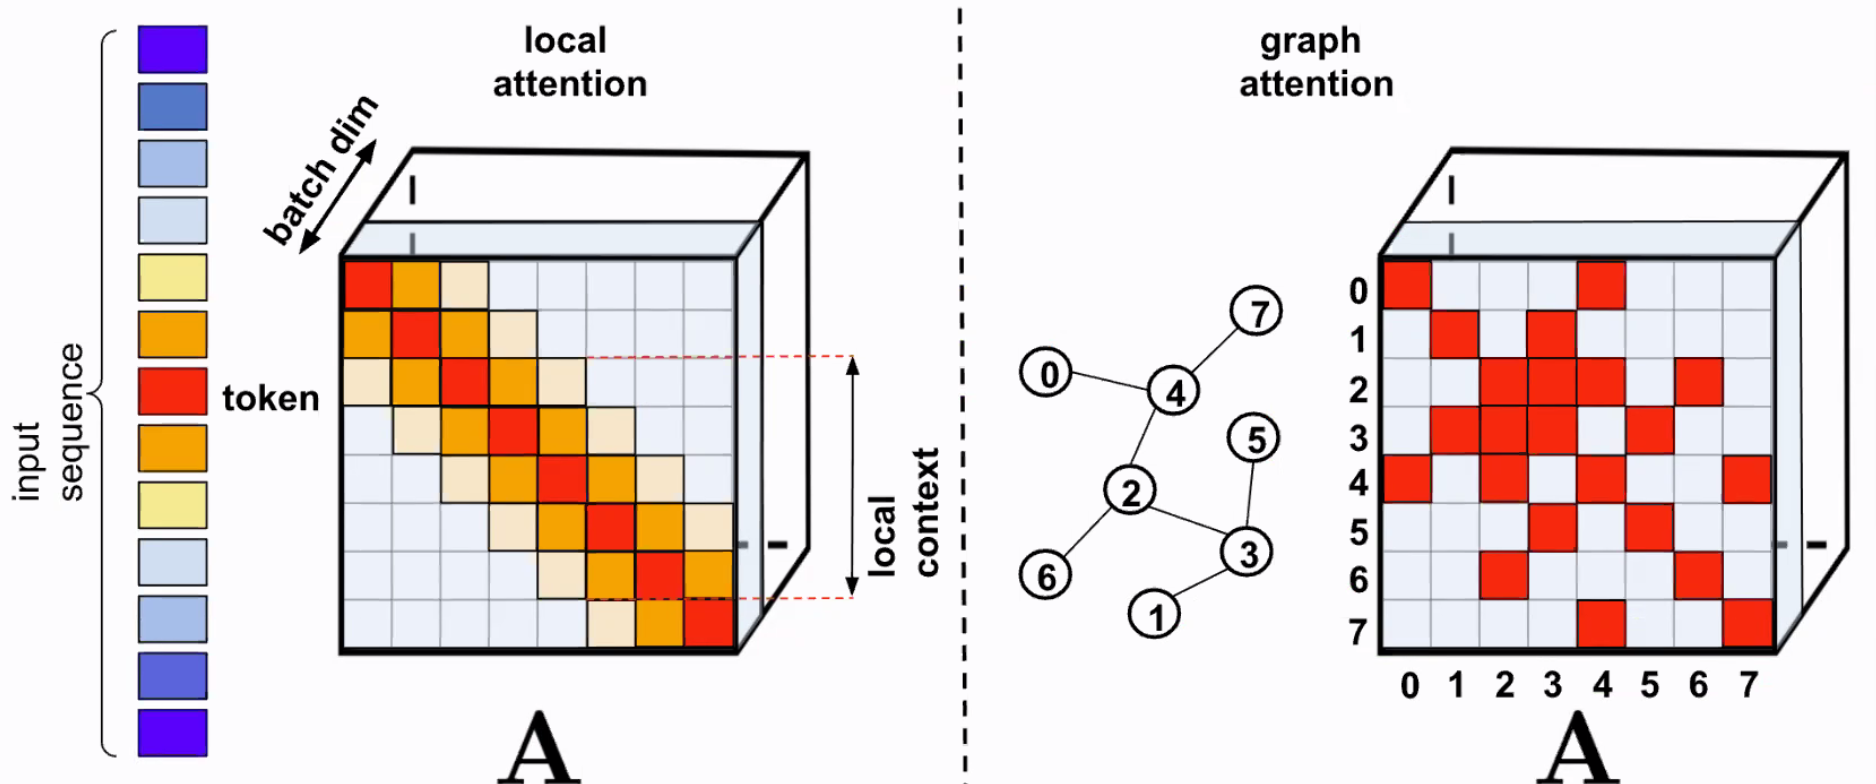
\includegraphics[width=0.9\textwidth]{local_attention.png}

One way to make the attention architecture more scalable would be to only look at local attention, or attention in the neighborhood of each token. Graph attention is another possibility. 	

We talked about how the  attention matrix could roughly be though of as a similarity matrix. In ML, we refer to similarity matrices as kernels. 


\subsubsection*{Terms to look up:}
\begin{itemize}
	\item dense attention vs. sparse attention
	\item attend (verb)
	\item attention matrix
	\item queries and keys in attention
	\item performer model
	\item kernelizable in ``attention is kernelizable''. Also, \href{https://en.wikipedia.org/wiki/Kernel_method}{kernel methods} in general
	\item partition function 
\end{itemize}


Usually, you take some row representation of you data.
\chapter{Transformers (cont.) [Lec. 5]}
Feb. 22


\subsubsection*{Positional encoding}

\href{https://paperswithcode.com/paper/attention-is-all-you-need}{Attention Is All You Need}. 
This section refers to positional encoding 
You have a positional encoding, add it to your one hot vector. That's how you encode time. That's how you encode positions in your sequence. 

Enriched row embedding

Gieven $x_t$, a one-hot vector, and $f(t)$, where $t$ is a positional encoding. We add $x_t + f(t)$. 

\subsubsection*{Multiple-head mechanism}

\begin{itemize}
	\item \href{https://paperswithcode.com/method/multi-head-attention}{Multi-Head Attention [article] - Lilian Weng}
	\item \href{https://github.com/jadore801120/attention-is-all-you-need-pytorch/blob/fec78a687210851f055f792d45300d27cc60ae41/transformer/SubLayers.py#L9}{[PyTorch code]}
\end{itemize}

Multi-head Attention is a module for attention mechanisms which runs through an attention mechanism several times in parallel. The independent attention outputs are then concatenated and linearly transformed into the expected dimension. Intuitively, multiple attention heads allows for attending to parts of the sequence differently (e.g. longer-term dependencies versus shorter-term dependencies). 
\begin{gather}
	\text{MultiHead}(Q, K, V) = H W_0 \\
	H = [h_1, \ldots, h_h], \quad h_i = \text{Attention}(QW_i^Q, KW_i^K, VW_i^V)
\end{gather}
The above $W$ terms are learnable parameter matrices and $h_i$ denotes the $i$th ``head''. Note that scaled dot-product attention is most commonly used in this module, although in principle, it can be swapped out for other types of attention mechanism. 

The multi-head attention mechanism was introduced by Vaswani et al. in \href{https://paperswithcode.com/paper/attention-is-all-you-need}{Attention Is All You Need}.


$L$ is the length of the sequence, $b$ is the batch dim, and $d$ is the dimensionality of the token embedding. The data is an $L \times b\times d$ tensor. 

As in standard NNs, transformers process data in batches. 

The idea of multiple-head attention is to use a couple different attention models in parellel.  

If you take a specific attention model, what you're essentially doing is learning 3 matrices, $W_Q, W_X,$ and $W_V$. Let $\mathcal{T}$ be the space of tensors. $W_Q \in \mathcal{T}_{L\times d_{QK} \times b}, W_K \in \mathcal{T}_{L \times d_{QK} \times b }, W_V \in \mathcal{T}_{L \times d \times b }$.  


\subsubsection*{Terms to look up:}
\begin{itemize}
	\item positional encoding
	\item mutliple-head mechanism
\end{itemize}

\chapter{The Unreasonable Effectiveness of ES}

A Tale of Hadamard-Minitaurs and Toeplitz-Walkers.

Fancy finite difference replacing backpropagation



\bibliography{master_references}

%%%%%%%%%%%%%%%%%%%%%%%%%

\end{document}

% Template Recipes

%Bold Text:
%	\textbf{}

%Inline code:
%	\lstinline{code}

%Note environment:
%	\begin{note}
%
%	\end{note}

%Remark environment:
%	\begin{remark}
%	  On Overleaf, please use \hologo{XeLaTeX} to compile articles in Chinese and \hologo{pdfLaTeX} to compile articles in English.
%	\end{remark}

%Listing (code) environment.
%	\begin{lstlisting}
%	tlmgr update --self
%	tlmgr update --all
%	print("hello world")
%	\end{lstlisting}

%Assumption environment:
%	\begin{assumption}
%		assumptions
%	\end{assumption}

% Acknowledgement
%- The `cls` file for my latex notes came from [ElegantLaTeX](https://elegantlatex.org/):  | [Github](https://github.com/ElegantLaTeX/ElegantBook) | [CTAN](https://ctan.org/pkg/elegantbook) | [Download](https://github.com/ElegantLaTeX/ElegantBook/releases) | [Wiki](https://github.com/ElegantLaTeX/ElegantBook/wiki).